
\begin{center}
\Huge
Forberedelse til prøve
\end{center}

\section*{Opgave 1}
Differentiér følgende funktioner
\begin{align*}
	&1) \ 2x^2+4x+1    &&2) \ 4\ln(x)    \\
	&3) \  3x^7   &&4) \ \frac{\sqrt{x}}{2}    \\
\end{align*}

\section*{Opgave 2}

\begin{enumerate}[label=\roman*)]
	\item Bestem ligningen for tangenten til funktionen $f$ givet ved
	\begin{align*}
		f(x) = x^2-2x+5
	\end{align*}
	i punktet $P(-2,f(-2))$
\end{enumerate}

\section*{Opgave 3}
En funktion $f$ er givet ved
\begin{align*}
	f(x) = \frac{1}{3}x^3+\frac{1}{2}x^2-6x+2
\end{align*}
\begin{enumerate}[label=\roman*)]
	\item Bestem $f'(x)$.
	\item Løs ligningen $f'(x) = 0$.
	\item Bestem monotoniforholdene for funktionen $f$ givet ved
	\begin{align*}
		f(x) = \frac{1}{3}x^3 + \frac{1}{2}x^2 -6x +2.
	\end{align*}
\end{enumerate}

\section*{Opgave 4}
På Fig. \ref{fig:grafer} kan graferne for en funktion $f$ samt dens afledede $f'$ ses.

\begin{figure}[H]
		\centering
		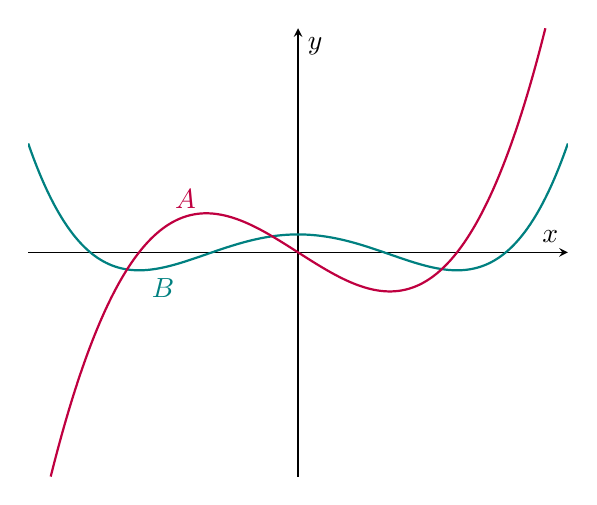
\begin{tikzpicture}
			\begin{axis}[
			axis lines = middle, 
			xlabel = {$x$},
			ylabel = {$y$},
			xmin = -2.4, xmax = 2.4,
			ticks = none]
				\addplot[color = teal, samples = 1000, thick, domain = -2.4:2.4] {x^4-4*x^2+2};
				\addplot[color = purple, samples = 1000, thick, domain = -2.2:2.2] {4*x^3-8*x};
				\node[color = purple] at (axis cs: -1,6) {$A$};
				\node[color = teal] at (axis cs: -1.2,-4) {$B$};
			\end{axis}
		\end{tikzpicture}
		\caption{Grafer for $f$ og $f'$}
		\label{fig:grafer}
\end{figure}

\begin{enumerate}[label=\roman*)]
	\item Afgør hvilken af graferne der tilhører $f$ og hvilken der tilhører $f'$. Begrund dit svar. 
\end{enumerate}

\section*{Opgave 5}
Differentiér følgende.
\begin{align*}
	&1) \ x^2\cdot \sqrt{x}   &&2) \ln(x)\cdot x-x    
\end{align*}

